\part{Analysis}
		\section{Problem Identification}
		\section{Literature Review}
			This section aims to explore the key elements of the project with justification for their usage accompanied by relevant literature.
			
			\subsection{SLAM}
				\subsubsection{What is SLAM?}
				SLAM stands for Simultaneous Localization and Mapping, and is something sometimes employed by mobile robots. Localization refers to the ability for the robot to be aware of its location within an environment, for example knowing where it is within a room. Mapping simply refers to building a map of the environment, such as the room the robot is in. SLAM is performing both of these tasks at the same time. Hugh Durrant-Whyte and Tim bailey, both engineers reknowned for their exceptional work in robotics best sum it up in this IEEE entry as the ability for a mobile robot to be placed at an unknown location in an unknown environment and then both create a consistent map of the environment and be able to accurately determine its location within this map \citep{durrant2006simultaneous}. Similar definitions can also be found in other articles \citep{choset2001topological, dissanayake2001solution}.
			
				\subsubsection{Uses of SLAM}
				SLAM allows for autonomous robots to function in unknown environment \citep{durrant2006simultaneous, dissanayake2001solution}, and as such there are a myriad of potential uses, many of which can be seen within the wider industry. Commercially it has been used for products such as vacuum cleaners, Dyson for instance has a small automated vacuum cleaner called the 360 Eye which employs SLAM techniques to map the areas that it moves around and cleans. SLAM has seen many uses in archaeological contexts owing to its ability to perform exploration without risk to human life, one team \citep{clark2008archaeology} developed an underwater robot that used SLAM in order to map underwater cisterns that had been built thousands of years ago. The uses have not gone unnoticed by larger organisations. One of the research organisations within the USA?s Department of Defense has held challenges (known as the DARPA Grand Challenge) offering cash prizes as incentives to create high value research. These challenges involve organisations submitting cars that are timed as they race around certain environments. NASA have also made use of it in the past, in 2007 they used an autonomous underwater robot \citep{carnegie2007sinkhole} employing SLAM to go to the bottom of the world's deepest sinkhole. The robot used sensors to generate a sonar map of the sinkhole's inner dimensions 318 meters below the surface.  The drone also tested technologies that could be used in other more extreme underwater environments such as the oceans under the crust of Europa, one of Jupiter's moons. Interest has also been expressed in using SLAM for planetary rovers, allowing for the mapping and navigation of different planet surfaces.
				\medskip
			
				\subsubsection{The SLAM Problem}
				Let's use some key notations to help break down the essentials of the SLAM problem. \newline
				\textbf{k} - Current time. \newline
				\textbf{x\textsubscript{k}} - Location and orientation of vehicle. \newline
				\textbf{u\textsubscript{k}} - Control vector, for example drive forward 1 metre.  \newline
				\textbf{m\textsubscript{i}} - True location of \textit{i}th landmark within the environent. \newline
				\textbf{z\textsubscript{ik}} - Observation of \textit{i}th landmark taken at time \textit{k}.\newline
				
				From these notations we can derive some sets. \newline
				\textbf{x\textsubscript{0:k}} = $\lbrace$ \textbf{x\textsubscript{0:k-1}}, \textbf{x\textsubscript{k}} $\rbrace$ - History of all vehicle locations. \newline
				\textbf{u\textsubscript{0:k}} = $\lbrace$ \textbf{u\textsubscript{0:k-1}}, \textbf{u\textsubscript{k}} $\rbrace$ - History of all control inputs. \newline
				\textbf{m} = $\lbrace$ \textbf{m\textsubscript{1}}, \textbf{m\textsubscript{2}}, ..., \textbf{m\textsubscript{n}}$\rbrace$ - Set of all landmarks. \newline
				\textbf{z\textsubscript{0:k}} = $\lbrace$ \textbf{z\textsubscript{0:k-1}}, \textbf{z\textsubscript{k}} $\rbrace$ - Set of all landmark observations. \newline
				
				Ultimately we want to use the robot's control inputs and observations to receive a map of the environment and the robot's path. Landmark measurements would be gained by an appropriate medium, such as a LIDAR sensor. Robot locations can be achieved a few different ways. One of the more straightforward methods for this is simply using a robot's control vectors, having its internal position modified by the different movement commands it receives. More sophisticated robots may use odometry, which involves using data from motion sensors. One of the more common examples of this is through the use of wheel encoders, where the robot can track wheel revolutions and use this to estimate distance.
			
				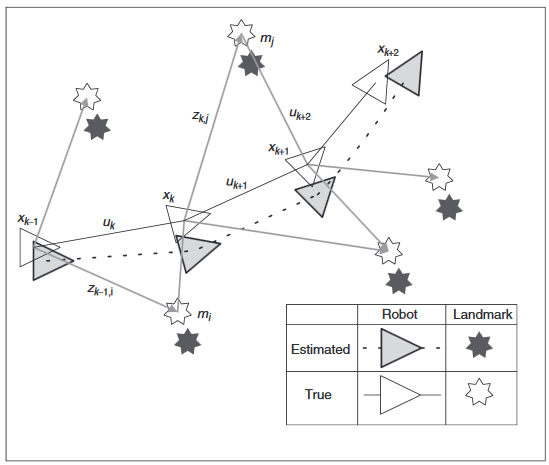
\includegraphics[scale=0.65]{ANALYSIS/slamdiagram.png} \newline
				The SLAM problem illustrated \citep{durrant2006simultaneous}.
			
				\medskip
				
				\subsubsection{SLAM Taxonomy}
				Whilst the term SLAM refers to one encompassing concept, there is not necessarily one encompassing SLAM issue affecting all situations where it could be used. Below are some common variants within the SLAM problem.
				
					\paragraph{Volumetric versus Feature-Based}
					Volumetric SLAM samples the map as a resolution high enough to allow a photo realistic reconstruction of the environment \citep{thrun2008simultaneous}. The map gained from this is generally high dimensional, but as the area increases in size and scale the map becomes significantly more complex. Feature-based SLAM simply extracts key features from measurements, with the map being solely made up of these features. This might be used if it is decided that only key features are of interest or if large parts of the mapped space are empty, as volumetric SLAM in these cases would be storing voxels that hold no geometric data of significant value \citep{vespa2018efficient}. As you would expect, this is quicker and more efficient but discards a lot more data than volumetric. 
					
					\paragraph{Topological versus Metric}
					Topological SLAM captures key places and their connectivity to other measured locations. Metric SLAM attempts to model the environment using geomatrically accurate positioning. Metric SLAM would show the accurate positioning of various environmental features, topological would show them in relation to eachother (e.g. place A is adjacent to place B) \citep{thrun2008simultaneous}.
					
					\paragraph{Known versus Unknown Correspondence}
					
					
					\paragraph{Static versus Dynamic}
					Static and Dynamic here refers to the environment. Static SLAM assumes an unchanging environment, Dynamic SLAM has features that accommodate for the environment changing.
					
					\paragraph{Small versus Large Uncertainty}
					
					
					\paragraph{Activate versus Passive}
					Active SLAM involves the robot actively exploring its environment whilst it builds a map of it. Passive SLAM is when the SLAM algorithm is purely used for observation, with some other entity controlls the robot's movement. 
					
					\paragraph{Single-Robot versus Multirobot}
					Single-robot simply refers to SLAM happening only on a single platform. Multirobot SLAM (sometimes known as cooperative SLAM) involves multiple robots often communicating with eachother to merge their maps into a larger collective model. 
				
			
				\subsubsection{Solutions}
				SLAM is generally approached probabilistically. This means that the attempted solutions factor in uncertainties within the data. Therefore, solutions to the SLAM problem will not act with exact certainties. For example, rather than saying the robot is in an exact location we would treat it as a general location it is the most likely to be in. This can be summed up as -
				
				p (\textbf{x\textsubscript{0:k}}, \textbf{m} $\mid$ \textbf{z\textsubscript{0:k}}, \textbf{u\textsubscript{0:k}})
				
				We want the probability distribution to be an estimation of what is on the left (current vehicle location and landmarks) based on what's on the right (landmark observations and control inputs). There are different approaches to the implementation of this, but three stand out as the most major. % am i explaining individual SLAM implementations?
			
			\subsection{LIDAR}
				\subsubsection{What is LIDAR?}
					LIDAR (Light Detection And Ranging) is a technology that uses light sensors to measure distances between the sensor and the target object. It achieves this by sending out light pulses which bounce off of objects back at the sensor where they are collected.
					
				
				\subsubsection{Uses of LIDAR}
				
			

		\section{Solutions}
		\section{Product Requirements}
			
		
		
		\section{Review of Tools and Techniques}
			\subsection{Scanning Behaviour}
			One aspect that needed to be considered was the drone's behaviour whilst scanning. The initial thought was that the drone would move around, scan and save the scan results all simultaneously. To investigate the viability of this tests were performed to see if this was possible with the constraints we had, the most notable constraints being how quickly the MBed board is able to write scan data compared to how quickly it would be receiving it from the LIDAR sensor. *!Have some numbers here describing the time it takes to write data retrieved from 1 seconds' worth of LIDAR scanning!*. Based on this it was decided it would be best if the LIDAR stopped and took readings for a small period of time, with these readings being stored in the RAM and then written to internal files afterward. 
			
			\subsection{Dead Reckoning}
			Odometry is the usage of data from motion sensors to estimate an object's position. One such implementation of this that will be looked at for the project is dead reckoning. Dead reckoning tracks the robot's position by using data from wheel encoders that count the number of wheel rotations performed during operation. From this, the internal tracked position of a robot can estimate its new position after periods of movement. Given that the chassis being used for the project has wheel encoders as part of the wheel motors, this approach would allow us to perform odometry without needing the use of additional kit. Dead reckoning is not without issues however. Most pressingly it does not account for wheel slippage. If the robot has a poor grip on the ground and the wheels slip, then the wheel rotation doesn't accurately correspond to the robot's location \citep{choset2001topological}. These issues would compound as well. As more and more slippage happens, the robot's internal position would become less and less accurate to where it actually is.
				
	